%*****************************************
\chapter{Experimental Research}\label{ch09:experimental_research}
%*****************************************
%TODO Status: Pre-draft

\section{Introduction}

\begin{wrapfigure}{r}{0.4\textwidth}
	\centering
	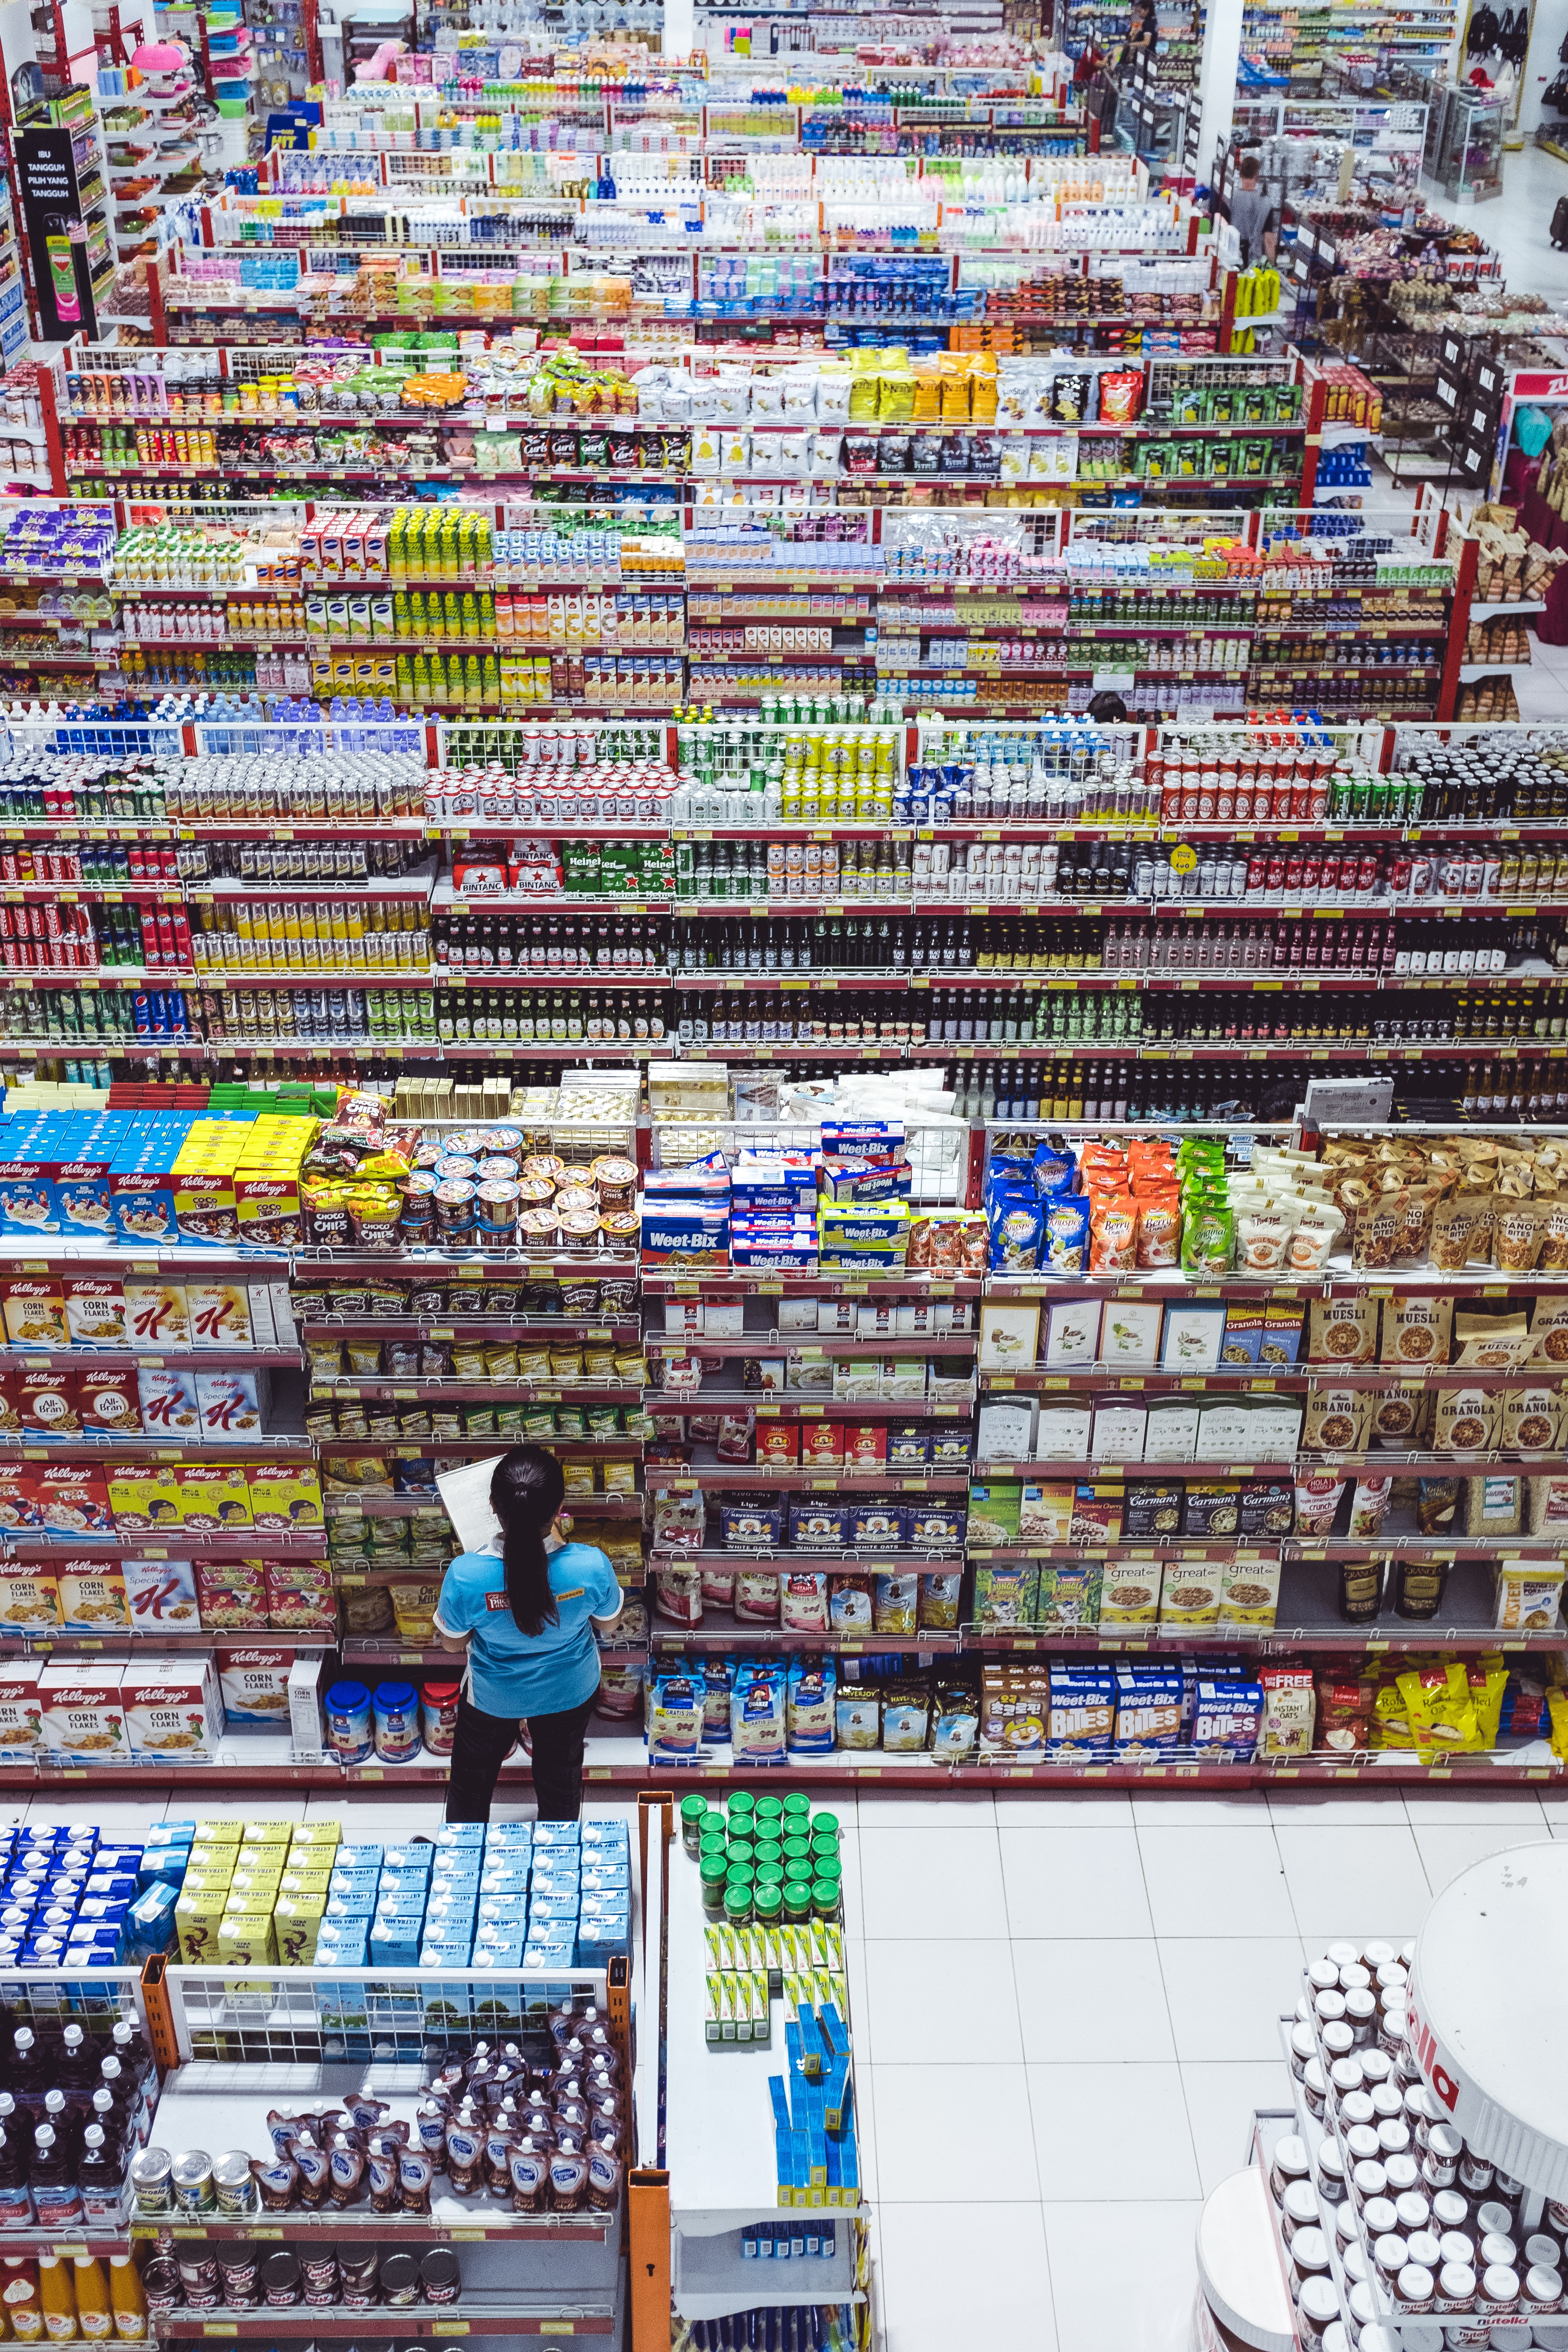
\includegraphics[width=0.4\textwidth]{gfx/09-experiment} 
\end{wrapfigure}

With thousands of products to sell, how does a merchant determine what to stock? Often that decision is the result of an experiment. The merchant may stock two or three similar items and then check to see what sells best. Part of the experiment may include manipulating the price of the items, their locations in the store, and how they are advertised. In the end, the merchant would have generated solid data to help determine what products to stock in the future.\blfootnote{Photo by Bernard Hermant on Unsplash}

Experimental research, often considered to be the ``gold standard'' in research designs by researchers who are \gls{positivist} in outlook, is one of the most rigorous of all research designs. In this design, one or more independent variables are manipulated by the researcher (``treatments''), subjects are randomly assigned to different treatment levels, and the results of the treatments on outcomes are observed and analyzed. The unique strength of experimental research is its \gls{internalvalidity} due to its ability to link cause to an effect through treatment manipulation while controlling for the spurious effect of extraneous variables.

\begin{center}
	\begin{objbox}{Objectives}
		\begin{itemize}
			\setlength{\itemsep}{0pt}
			\setlength{\parskip}{0pt}
			\setlength{\parsep}{0pt}
			
			\item Describe experimental research
			\item Define the terms control group, treatment group, treatment manipulation, random selection, validity
			\item Describe how internal validity can be improved
			\item Describe two-group designs
			\item Describe factorial designs
			\item Describe hybrid designs
			\item Describe quasi-experimental designs
			\item List the strengths and weaknesses of experimental formats
		\end{itemize}
	\end{objbox}
\end{center}

One example of experimental research can be found in Alcott's study of behavioral interventions\cite{allcott2014short}. In this study, the results of the \textit{Opower} program were evaluated. Opower was a company that sent a ``home energy report'' to more than six million homes representing $ 85 $ utilities across the United States. The reports were designed to use social pressure to get homeowners to moderate their electricity use. For Alcott's experiment, the three different sites were compared using pre- and post- intervention electricity usage statistics. He found that the initial home energy report caused high-frequency ``action and backsliding,'' but the cycles seem to attenuate over time. He also found that if the reports were discontinued the effect was still relatively persistent. Finally, he found that consumers are slow to habituate. While this study was focused on a single intervention involving energy conservation, it may be interesting to speculate if similar intervention efforts in areas like dieting, exercise, and smoking cessation would experience similar results.

Experimental research is best suited for \gls{explanatoryresearch}, where the goal of the study is to examine cause-effect relationships, rather than for descriptive or \gls{exploratoryresearch}. It also works well for research that involves a relatively limited and well-defined set of independent variables that can either be manipulated or controlled. The conduct of experimental research is generally found in one of two settings. 

\begin{itemize}
	\item Laboratory experiments, conducted in laboratory (artificial) settings, tend to be high in \gls{internalvalidity}, but this comes at the cost of low \gls{externalvalidity} because the artificial setting in which the study is conducted may not reflect the real world. As one example of a laboratory study, Berger and Iyengar\cite{berger2013communication} studied how the medium, oral vs. written, shapes the message in word-of-mouth communications. As part of their research, they conducted three laboratory studies and then collected field data to validate the laboratory studies. They found that there was a difference in how people communicated about brand name products when the channel was oral rather than written. They found, specifically, that written communication (like online chat) led to people mentioning more interesting products and brands than when they talked about them orally.

	\item Field experiments, conducted in field settings such as in an organization, can be high in \gls{externalvalidity}. But such experiments are relatively rare, because of the difficulties associated with manipulating treatments and controlling for extraneous effects in a field setting. As an example of a field experiment, Cai, Chen, and Fang\cite{cai2009observational} observed diners in restaurants to determine if knowing what other people had ordered influenced what they in turn ordered. They found that the demand for the top five dishes was increased by about $ 13 - 18\% $ when the popularity ratings were revealed to customers. 
\end{itemize}

It is common for researchers to combine experimentation settings in one project so the results of one setting can be validated in another setting. Gainsbury and Blaszczynski\cite{gainsbury2011appropriateness} specifically researched the question of whether laboratory and field experiments came to the same result. They set up a gambling laboratory and had $ 127 $ students play an electronic gambling machine that included warning about gambling presented in two different ways: pop-up and static sign. They then interviewed the gamblers to see what they remembered about the warnings. Then they went to a casino and repeated the experiment with gamblers who happened to be present. They found that the ``venue participants'' were less likely to complete surveys and when they did they provided less information than the laboratory participants. They concluded that while both settings provided valuable information about gambling behavior, care must be taken in generalizing the laboratory results to the ``real world.''

Experimental research designs can be grouped into two broad categories: true and quasi-experimental designs. Both designs require the manipulation of a treatment, but true experiments also require random assignment of participants while quasi-experiments do not. As an example of a quasi-experiment, McElroy and Morrow\cite{mcelroy2010employee} evaluated the result of an office redesign project in a large financial services company. They compared two groups of employees, those who were reassigned to a new office design and those who were not. They surveyed $ 127 $ employees who had moved and $ 144 $ who had not and then compared the perceptions of the work space and organization's culture for both groups. They found that those who moved reported less workspace and more distractions than those who did not, but the results varied by the age of the respondent. They also reported more favorable perceptions of the organization's culture and work-related attitudes with no age difference. Because the participates had not been randomly assigned to groups this was a quasi-experimental design.

\section{Basic Concepts}

All experimentation designs include the following characteristics.

\paragraph{Treatment and control groups.} In experimental research, some subjects are administered one or more experimental stimulus called a treatment (the treatment group) while other subjects are not given such a stimulus (the control group). The treatment may be considered successful if subjects in the treatment group rate more favorably on outcomes than control group subjects. Multiple levels of experimental stimulus may be administered, in which case there may be more than one treatment group. For example, in order to test the effectiveness of an advertisement, researchers may expose three different groups of people to different levels of advertising. One treatment group would view a printed article with an embedded advertisement, a second treatment group would view a television program with an embedded advertisement, and the third group, the control group, would view media with no advertising. After the exposure period, the groups could be surveyed to determine which remembered the advertising best.

\paragraph{Treatment manipulation.} Treatments are the unique feature of experimental research that sets this design apart from all other research methods. Treatment manipulation helps control for the ``cause'' in cause-effect relationships. Treatments must be checked using various pilot tests prior to the start of the experiment. Any measurements conducted before the treatment is administered to the subjects are called pretest measures and those conducted after the treatment are post-test measures. 

\paragraph{Random selection and assignment.} Random \textit{selection} is the process of randomly drawing a sample from a population or a sampling frame. This approach is typically employed in survey research and assures that each unit in the population has an equal chance of being selected into the sample. Random \textit{assignment} is the process of randomly assigning subjects to experimental or control groups. This is a standard practice in true experimental research to ensure that treatment groups are similar to each other and to the control group prior to treatment administration. Random selection is related to sampling, and is therefore, more closely related to the \gls{externalvalidity} of findings while random assignment is related to design and is related to \gls{internalvalidity}. It is common to include both random selection and random assignment in well-designed experimental research.

\paragraph{Threats to internal validity.} Although experimental designs are considered more rigorous than other research methods in terms of the internal validity of their inferences (by virtue of their ability to control causes through treatment manipulation), they are not immune to internal validity threats. As an example, imagine that researchers wanted to study the effect of a special mathematics tutoring program. They would want to plan for the following internal validity threats.

\begin{itemize}
	\item \textit{History threat} is the possibility that the observed outcomes (dependent variables) are caused by extraneous or historical events rather than by the experimental treatment. For instance, students' post-tutoring mathematics score improvement may have been caused by their preparation for a mathematics examination rather than the tutoring program.

	\item \textit{Maturation threat} refers to the possibility that observed effects are caused by natural maturation of subjects (\eg, a general improvement in their intellectual ability to understand complex concepts) rather than the experimental treatment. Perhaps the mathematics students' post-tutoring scores improved merely because they matured during the study and were better able to understand mathematics concepts.

	\item \textit{Testing threat} is a threat in pre/post designs where subjects' post-test responses are conditioned by their pretest responses. For instance, if students remember their answers from the pretest evaluation they may be able to repeat them in the post-test exam.

	\item \textit{Instrumentation threat} refers to the possibility that the difference between pretest and post-test scores is not due to the mathematics tutoring program but, rather, to changes in the administered test, such as the post-test having a higher or lower degree of difficulty than the pretest.

	\item \textit{Mortality threat} refers to the possibility that subjects may be dropping out of the study due to a systematic reason not necessarily related to the treatment. If the low-performing students drop out, the results of the post-test will be artificially inflated by the preponderance of high-performing students.

	\item \textit{Regression threat}, also called a ``regression to the mean,'' refers to the statistical tendency of a group's overall performance on a measure during a post-test to regress toward the mean of that measure rather than in the anticipated direction. For instance, if students in the mathematics study scored high on the pretest, they will have a tendency to score lower on the post-test (closer to the mean) because their initial high scores could have been a statistical aberration. It would also be true that students who under-performed on the pretest would tend to score closer to the mean on the post-test, which would falsely appear to be due to the tutoring treatment.
\end{itemize}

\section{Two-Group Experimental Designs}

The simplest true experimental designs are two group designs involving one treatment group and one control group, and are ideally suited for testing the effects of a single independent variable that can be manipulated as a treatment. The two basic two-group designs are the pretest/post-test control group design and the post-test-only control group design, while variations may include covariance designs. These designs are often depicted using a standardized design notation, where \textit{R} represents random assignment of subjects to groups, \textit{X} represents the treatment administered to the treatment group, and \textit{O} represents pretest or post-test observations of the dependent variable (with different subscripts to distinguish between pretest and post-test observations of treatment and control groups).

\paragraph{Pretest/post-test control group design.} In this design, subjects are randomly assigned to treatment and control groups, subjected to an initial (pretest) measurement of the dependent variables of interest, the treatment group is administered a treatment (representing the independent variable of interest), and the dependent variables measured again (post-test). The notation of this design is shown in Table \ref{09:tab01}, where each group's process should be read from left-to-right. Thus, the Treatment Group (top line) is first assigned using a random process, then a pretest is administered (Observation 1), then a treatment of some sort is applied, finally, a post-test is administered. The Control Group (bottom line) follows the same process, except there is no treatment applied.

\begin{table}[H]
	\centering
	\begin{tabularx}{0.85\linewidth}{p{0.10\linewidth}p{0.10\linewidth}p{0.10\linewidth}p{0.10\linewidth}p{0.40\linewidth}}
		\toprule
		\textit{R} & $ O_1 $ & \textit{X} & $ O_2 $ & \textsc{Treatment Group} \\
		\textit{R} & $ O_3 $ &            & $ O_4 $ & \textsc{Control Group} \\
		\bottomrule
	\end{tabularx}
	\caption{Pretest/Post-test Design}
	\label{09:tab01}
\end{table}

The effect, \textit{E}, of the experimental treatment in the pretest post-test design is measured as the difference in the post-test and pretest scores between the treatment and control groups, as shown in Equation \ref{09:eq01}

\begin{align}
	\label{09:eq01}
	E = (O_2 – O_1) – (O_4 – O_3)
\end{align}

Statistical analysis of this design involves a simple \gls{anova} between the treatment and control groups. The pretest post-test design mitigates several threats to internal validity, such as maturation, testing, and regression, since these threats can be expected to influence both treatment and control groups in a similar random manner. The selection threat is controlled via random assignment of members. However, additional threats to internal validity may exist. For instance, mortality can be a problem if there are differential dropout rates between the two groups, and the pretest measurement may bias the post-test measurement (especially if the pretest introduces unusual topics or content).

\paragraph{post-test-only control group design.} This design is a simpler version of the pretest/post-test design where pretest measurements are omitted. The design notation is shown in Table \ref{09:tab02}.

\begin{table}[H]
	\centering
	\begin{tabularx}{0.90\linewidth}{p{0.15\linewidth}p{0.15\linewidth}p{0.15\linewidth}p{0.40\linewidth}}
		\toprule
		\textit{R} & \textit{X} & $ O_1 $ & \textsc{Treatment Group} \\
		\textit{R} &            & $ O_2 $ & \textsc{Control Group} \\
		\bottomrule
	\end{tabularx}
	\caption{Post-test Only Design}
	\label{09:tab02}
\end{table}

The treatment effect is measured simply as the difference in the post-test scores between the two groups, as shown in Equation \ref{09:eq02}

\begin{align}
	\label{09:eq02}
	E = (O_1 – O_2)
\end{align}

The appropriate statistical analysis of this design is also a two-group \gls{anova}. The simplicity of this design makes it more attractive than the pretest/post-test design in terms of internal validity. This design controls for maturation, testing, regression, selection, and pretest/post-test interaction, though the mortality threat may continue to exist.

\paragraph{Covariance designs.} Sometimes, the measure of a dependent variable may be influenced by an extraneous variable called a \gls{covariate}. Covariates are those variables that are not of central interest to an experimental study, but should nevertheless be controlled in order to eliminate their potential effect on the dependent variable and therefore allow for a more accurate detection of the effects of the independent variables of interest. A covariance design is a special type of pretest post-test control group design where the pretest measure is essentially a measurement of the covariates of interest rather than that of the dependent variables. The design notation is shown in Table \ref{09:tab03}, where \textit{C} represents the covariates:

\begin{table}[H]
	\centering
	\begin{tabularx}{0.85\linewidth}{p{0.10\linewidth}p{0.10\linewidth}p{0.10\linewidth}p{0.10\linewidth}p{0.40\linewidth}}
		\toprule
		\textit{R} & \textit{C} & \textit{X} & $ O_1 $ & \textsc{Treatment Group} \\
		\textit{R} & \textit{C} &            & $ O_2 $ & \textsc{Control Group} \\
		\bottomrule
	\end{tabularx}
	\caption{Covariate Design}
	\label{09:tab03}
\end{table}

Because the pretest measure is not a measurement of the dependent variable, but rather a covariate, the treatment effect is measured as the difference in the post-test scores between the treatment and control groups as in Equation \ref{09:eq03}.

\begin{align}
	\label{09:eq03}
	E = (O_1 – O_2)
\end{align}

Due to the presence of covariates, the right statistical analysis of this design is a two-group \gls{ancova}. This design has all the advantages of post-test only design, but with internal validity due to the controlling of covariates. Covariance designs can also be extended to pretest/post-test control group design.

\section{Factorial Designs}

Two-group designs are inadequate if the research project requires manipulation of two or more independent variables (treatments). In such cases, four or higher-group designs are required. Such designs, quite popular in experimental research, are commonly called \glspl{factorialdesign}. Each independent variable in this design is called a factor, and each sub-division of a factor is called a level. Factorial designs enable researchers to examine not only the individual effect of each treatment on the dependent variables (called main effects), but also their joint effect (called interaction effects).

The most basic factorial design is a $ 2 x 2 $ factorial design, which consists of two treatments, each with two levels (such as high/low or present/absent). For instance, suppose a research project compares the learning outcomes of two different types of instructional techniques (online and in-class) along with the time of instruction ($ 1.5 $ or $ 3 $ hours per week). In this case, there are two factors: instructional type and instructional time; each with two levels (in-class and online for instructional type, and $ 1.5 $ and $ 3 $ hours/week for instructional time), as shown in Figure \ref{09:fig01}. If a third level of instructional time (maybe $ 6 $ hours/week) is desired then the second factor will consist of three levels and a $ 2 x 3 $ factorial design is required. On the other hand, if a third factor, such as group work (present versus absent), is desired, then a $ 2 x 2 x 2 $ factorial design is needed. In this notation, each number represents a factor, and the value of each factor represents the number of levels in that factor.

\begin{center}
	\begin{figure}[H]
		\tikzstyle{tlbox}=[rectangle,draw=blue!50,fill=blue!20,ultra thick,
		inner sep=10pt,minimum width=4.5cm,minimum height=2.0cm,
		rounded corners=.25cm]
		\tikzstyle{trbox}=[rectangle,draw=red!50,fill=red!20,ultra thick,
		inner sep=10pt,minimum width=4.5cm,minimum height=2.0cm,
		rounded corners=.25cm]
		\tikzstyle{blbox}=[rectangle,draw=green!50,fill=green!20,ultra thick,
		inner sep=10pt,minimum width=4.5cm,minimum height=2.0cm,
		rounded corners=.25cm]
		\tikzstyle{brbox}=[rectangle,draw=yellow!50,fill=yellow!20,ultra thick,
		inner sep=10pt,minimum width=4.5cm,minimum height=2.0cm,
		rounded corners=.25cm]			
		\tikzstyle{every label}=[red]
		\begin{tikzpicture}
		\node[tlbox] (gp1)                      {Group 1};
		\node[trbox] (gp2) [right=0.5cm of gp1] {Group 2};
		\node[blbox] (gp3) [below=0.5cm of gp1]	{Group 3};
		\node[brbox] (gp4) [right=0.5cm of gp3] {Group 4};
		
		\node[] (ttext1) [above=1.0cm of gp1,xshift=2.5cm] {Instructional Time};
		\node[] (ttext2) [above=0.5cm of gp1,yshift=-0.25cm] {1.5 hours/wk};		
		\node[] (ttext3) [above=0.5cm of gp2,yshift=-0.25cm] {3.0 hours/wk};		
		\node[] (ltext1) [left=1.0cm of gp1,yshift=0.50cm,rotate=90] {Instructional Type};
		\node[] (ltext2) [left=0.5cm of gp1,yshift=0.75cm,rotate=90] {Online};
		\node[] (ltext3) [left=0.5cm of gp3,yshift=0.75cm,rotate=90] {In-class};
		
		\node[] (factor) [red,left=3.0cm of ttext1] {Factors};
		\node[] (level)  [blue, left=2.5cm of ttext1,yshift=-0.68cm] {Levels};

		% Arrows		
		\draw [->,red,line width=1pt] (factor) to (ttext1);
		\draw (-3.25cm, 2.10cm) [->,red,line width=1pt] to (ltext1.east);
		\draw [->,blue,line width=1pt] (level) to (ttext2);
		\draw (-2.775cm, 1.30cm) [->,blue,line width=1pt] to (ltext2.east);
		
		
		\end{tikzpicture}
		\caption{2X2 Factorial Design}
		\label{09:fig01}
	\end{figure}
\end{center}

Factorial designs can also be depicted using a design notation, such as that shown in Table \ref{09:tab04}. 

\begin{table}[H]
	\centering
	\begin{tabularx}{0.75\linewidth}{p{0.15\linewidth}p{0.15\linewidth}p{0.15\linewidth}p{0.25\linewidth}}
		\toprule
		\textit{R} & $ X_{11} $ & $ O_1 $ & \textsc{Group 1} \\
		\textit{R} & $ X_{12} $ & $ O_2 $ & \textsc{Group 2} \\
		\textit{R} & $ X_{21} $ & $ O_3 $ & \textsc{Group 3} \\
		\textit{R} & $ X_{22} $ & $ O_4 $ & \textsc{Group 4} \\
		\bottomrule
	\end{tabularx}
	\caption{2X2 Factorial Design}
	\label{09:tab04}
\end{table}

\textit{R} represents random assignment of subjects to treatment groups, \textit{X} represents the treatment groups themselves (the subscripts of \textit{X} represents the level of each factor), and \textit{O} represent observations of the dependent variable. Notice that the $ 2 x 2 $ factorial design will have four treatment groups, corresponding to the four combinations of the two levels of each factor. Correspondingly, a $ 2 x 3 $ design will have six treatment groups, and a $ 2 x 2 x 2 $ design will have eight treatment groups. As a rule of thumb, each cell in a factorial design should have a minimum sample size of $ 20 $ (this estimate is derived from Cohen's power calculations based on medium effect sizes). So a $ 2 x 2 x 2 $ factorial design requires a minimum total sample size of $ 160 $ subjects, with at least $ 20 $ subjects in each cell. It is obvious that the cost of data collection can increase substantially with more levels or factors in a factorial design. Sometimes, due to resource constraints, some cells in such factorial designs may not receive any treatment at all, which are called \textit{incomplete factorial designs}, but incomplete designs decrease the ability to draw inferences about the those factors.

In a factorial design, a \textit{main effect} is said to exist if the dependent variable shows a significant difference between multiple levels of one factor and at all levels of other factors. No change in the dependent variable across factor levels is the null case (baseline), from which main effects are evaluated. In the above example, perhaps a main effect of instructional type, instructional time, or both can be seen on learning outcomes. An \textit{interaction effect} exists when the effect of differences in one factor depends upon the level of a second factor. In the above example, if the effect of instructional type on learning outcomes is greater for $ 3 $ hours/week of instructional time than for $ 1.5 $ hours/week, then there is an interaction effect between instructional type and instructional time on learning outcomes. Note that the presence of interaction effects dominate and make main effects irrelevant, and it is not meaningful to interpret main effects if interaction effects are significant.

\section{Hybrid Experimental Designs}

Hybrid designs are those that are formed by combining features of more established designs. Three such hybrid designs are randomized blocks design, Solomon four-group design, and switched replications design.

\paragraph{Randomized block design.} This is a variation of the post-test-only or pretest/post-test control group design where the subject population can be grouped into relatively homogeneous subgroups (called blocks) within which the experiment is replicated. For instance, to replicate the same post-test-only design among university students and full-time working professionals (two homogeneous blocks), subjects in both blocks are randomly split between a treatment group (receiving the same treatment) or control group (see Table \ref{09:tab05}). The purpose of this design is to reduce the ``noise'' or variance in data that may be attributable to differences between the blocks so that the actual effect of interest can be detected more accurately.

\begin{table}[H]
	\centering
	\begin{tabularx}{0.90\linewidth}{p{0.40\linewidth}p{0.15\linewidth}p{0.15\linewidth}p{0.15\linewidth}}
		\toprule
		\textsc{University Students} & \textit{R} & $ X $ & $ O_1 $ \\
		\textsc{University Students} & \textit{R} &       & $ O_2 $ \\
		\textsc{Professionals} & \textit{R} & $ X $ & $ O_3 $ \\
		\textsc{Professionals} & \textit{R} &       & $ O_4 $ \\
		\bottomrule
	\end{tabularx}
	\caption{Randomized Block Design}
	\label{09:tab05}
\end{table}

\paragraph{Solomon four-group design.} In this design, the sample is divided into two treatment groups and two control groups. One treatment group and one control group receive the pretest, and the other two groups do not. This design represents a combination of post-test-only and pretest/post-test control group design, and is intended to test for the potential biasing effect of pretest measurement on post-test measures that tends to occur in pretest/post-test designs but not in post-test only designs. The design notation is shown in Table \ref{09:tab06}.

\begin{table}[H]
	\centering
	\begin{tabularx}{0.65\linewidth}{p{0.15\linewidth}p{0.15\linewidth}p{0.15\linewidth}p{0.15\linewidth}}
		\toprule
		\textit{R} & $ O_1 $ & $ X $ & $ O_2 $ \\
		\textit{R} & $ O_3 $ &       & $ O_4 $ \\
		\textit{R} &         & $ X $ & $ O_5 $ \\
		\textit{R} &         &       & $ O_6 $ \\
		\bottomrule
	\end{tabularx}
	\caption{Solomon Four-group Design}
	\label{09:tab06}
\end{table}

\paragraph{Switched replication design.} This is a two-group design implemented in two phases with three waves of measurement. The treatment group in the first phase serves as the control group in the second phase, and the control group in the first phase becomes the treatment group in the second phase, as illustrated in Table \ref{09:tab07}. In other words, the original design is repeated or replicated temporally with treatment/control roles switched between the two groups. By the end of the study, all participants will have received the treatment either during the first or the second phase. This design is most feasible in organizational contexts where organizational programs (e.g., employee training) are implemented in a phased manner or are repeated at regular intervals.

\begin{table}[H]
	\centering
	\begin{tabularx}{0.75\linewidth}{p{0.10\linewidth}p{0.10\linewidth}p{0.10\linewidth}p{0.10\linewidth}p{0.10\linewidth}p{0.10\linewidth}}
		\toprule
		\textit{R} & $ O_1 $ & $ X $ & $ O_2 $ &       & $ O_3 $ \\
		\textit{R} & $ O_4 $ &       & $ O_5 $ & $ X $ & $ O_6 $ \\
		\bottomrule
	\end{tabularx}
	\caption{Switched Replication Design}
	\label{09:tab07}
\end{table}

\section{Quasi-Experimental Designs}

Quasi-experimental designs are almost identical to true experimental designs, but lacking one key ingredient: random assignment. For instance, one entire class section or one organization is used as the treatment group, while another section of the same class or a different organization in the same industry is used as the control group. This lack of random assignment potentially results in groups that are non-equivalent, such as one group possessing greater mastery of a certain content than the other group, say by virtue of having a better teacher in a previous semester, which introduces the possibility of selection bias. Quasi-experimental designs are therefore inferior to true experimental designs in interval validity due to the presence of a variety of selection related threats such as selection-maturation threat (the treatment and control groups maturing at different rates), selection-history threat (the treatment and control groups being impacted differently by extraneous or historical events), selection-regression threat (the treatment and control groups regressing toward the mean between pretest and post-test at different rates), selection-instrumentation threat (the treatment and control groups responding differently to the measurement), selection-testing (the treatment and control groups responding differently to the pretest), and selection mortality (the treatment and control groups demonstrating differential dropout rates). Given these selection threats, it is generally preferable to avoid quasi-experimental designs.

Many true experimental designs can be converted to quasi-experimental designs by omitting random assignment. For instance, the quasi-equivalent version of pretest/post-test control group design is called \gls{negd}, as shown in Table \ref{09:tab08}, with random assignment \textit{R} replaced by non-equivalent (non-random) assignment \textit{N}. Likewise, the quasi-experimental version of switched replication design is called \textit{Nonequivalent Switched Replication Design} (see Table \ref{09:tab09}).

\begin{table}[H]
	\centering
	\begin{tabularx}{0.85\linewidth}{p{0.10\linewidth}p{0.10\linewidth}p{0.10\linewidth}p{0.10\linewidth}p{0.40\linewidth}}
		\toprule
		\textit{N} & $ O_1 $ & \textit{X} & $ O_2 $ & \textsc{Treatment Group} \\
		\textit{N} & $ O_3 $ &            & $ O_4 $ & \textsc{Control Group} \\
		\bottomrule
	\end{tabularx}
	\caption{Nonequivalent Groups Design}
	\label{09:tab08}
\end{table}


\begin{table}[H]
	\centering
	\begin{tabularx}{0.75\linewidth}{p{0.10\linewidth}p{0.10\linewidth}p{0.10\linewidth}p{0.10\linewidth}p{0.10\linewidth}p{0.10\linewidth}}
		\toprule
		\textit{N} & $ O_1 $ & $ X $ & $ O_2 $ &       & $ O_3 $ \\
		\textit{N} & $ O_4 $ &       & $ O_5 $ & $ X $ & $ O_6 $ \\
		\bottomrule
	\end{tabularx}
	\caption{Nonequivalent Switched Replication Design}
	\label{09:tab09}
\end{table}

In addition, there are quite a few unique non-equivalent designs without corresponding true experimental design cousins, including those listed below.

\paragraph{\gls{rd} design.} This is a non-equivalent pretest/post-test design where subjects are assigned to treatment or control group based on a cutoff score on a pre-program measure. For instance, patients who are severely ill may be assigned to a treatment group to test the efficacy of a new drug or treatment protocol and those who are mildly ill are assigned to the control group. In another example, students who are lagging behind on standardized test scores may be selected for a remedial curriculum program intended to improve their performance, while those who score high on such tests are not selected from the remedial program. The design notation can be represented as in Table \ref{09:tab10}, where \textit{C} represents the cutoff score:

\begin{table}[H]
	\centering
	\begin{tabularx}{0.85\linewidth}{p{0.10\linewidth}p{0.10\linewidth}p{0.10\linewidth}p{0.10\linewidth}p{0.40\linewidth}}
		\toprule
		\textit{C} & $ O_1 $ & \textit{X} & $ O_2 $ & \textsc{Treatment Group} \\
		\textit{C} & $ O_3 $ &            & $ O_4 $ & \textsc{Control Group} \\
		\bottomrule
	\end{tabularx}
	\caption{Regression-discontinuity Design}
	\label{09:tab10}
\end{table}

Because of the use of a cutoff score, it is possible that the observed results may be a function of the cutoff score rather than the treatment, which introduces a new threat to internal validity. However, using the cutoff score also ensures that limited or costly resources are distributed to people who need them the most rather than randomly across a population, while simultaneously allowing a quasi-experimental treatment. The control group scores in the \gls{rd} design do not serve as a benchmark for comparing treatment group scores, given the systematic non-equivalence between the two groups. Rather, if there is no discontinuity between pretest and post-test scores in the control group, but such a discontinuity persists in the treatment group, then this discontinuity is viewed as evidence of the treatment effect.

\paragraph{Proxy pretest design.} This design, shown in Table \ref{09:tab11}, looks very similar to the standard \gls{negd} (pretest-post-test) design, with one critical difference: the pretest score is collected after the treatment is administered. A typical application of this design is when a researcher is brought in to test the efficacy of a program (\eg, an educational program) after the program has already started and pretest data is not available. Under such circumstances, the best option for the researcher is often to use a different prerecorded measure, such as students' grade point averages before the start of the program, as a proxy for pretest data. A variation of the proxy pretest design is to use subjects' post-test recollection of pretest data, which may be subject to recall bias, but nevertheless may provide a measure of perceived gain or change in the dependent variable.

\begin{table}[H]
	\centering
	\begin{tabularx}{0.85\linewidth}{p{0.10\linewidth}p{0.10\linewidth}p{0.10\linewidth}p{0.10\linewidth}p{0.40\linewidth}}
		\toprule
		\textit{N} & $ O_1 $ & \textit{X} & $ O_2 $ & \textsc{Treatment Group} \\
		\textit{N} & $ O_3 $ &            & $ O_4 $ & \textsc{Control Group} \\
		\bottomrule
	\end{tabularx}
	\caption{Proxy Pretest Design}
	\label{09:tab11}
\end{table}

\paragraph{Separate pretest/post-test samples design.} This design is useful if it is not possible to collect pretest and post-test data from the same subjects for some reason. As shown in Table \ref{09:tab12}, there are four groups in this design, but two groups come from a single non-equivalent group, while the other two groups come from a different non-equivalent group. For instance, to test customer satisfaction with a new online service that is implemented in one city but not in another, customers in the first city serve as the treatment group and those in the second city constitute the control group. If it is not possible to obtain pretest and post-test measures from the same customers, you can measure customer satisfaction at one point in time, implement the new service program, and measure customer satisfaction (with a different set of customers) after the program is implemented. Customer satisfaction is also measured in the control group at the same times as in the treatment group, but without the new program implementation. The design is not particularly strong, because changes in any specific customer's satisfaction score before and after the implementation cannot be examined, only the average customer satisfaction scores. Despite the lower internal validity, this design may still be a useful way of collecting quasi-experimental data when pretest and post-test data are not available from the same subjects.

\begin{table}[H]
	\centering
	\begin{tabularx}{0.65\linewidth}{p{0.15\linewidth}p{0.15\linewidth}p{0.15\linewidth}p{0.15\linewidth}}
		\toprule
		$ N_1 $ & $ O_1 $  &       &         \\
		$ N_1 $ &          & $ X $ & $ O_2 $ \\
		$ N_2 $ & $ O_3 $  &       &         \\
		$ N_2 $ &          &       & $ O_4 $ \\
		\bottomrule
	\end{tabularx}
	\caption{Separate Pretest/Posttest Samples Design}
	\label{09:tab12}
\end{table}

\paragraph{\gls{nedv} design.} This is a single-group pre/post quasi-experimental design with two outcome measures, where one measure is theoretically expected to be influenced by the treatment and the other measure is not. For instance, if a new calculus curriculum is being designed for high school students, the curriculum is anticipated to influence students' post-test calculus scores but not algebra scores. However, the post-test algebra scores may still vary due to extraneous factors such as history or maturation. Hence, the pre/post algebra scores can be used as a control measure, while the pre/post calculus scores can be treated as the treatment measure. The design notation, shown in Table \ref{09:tab13}, indicates the single group, \textit{N}, followed by pretest $ O_1 $ and post-test $ O_2 $ for both calculus and algebra for the same group of students. This design is weak in internal validity, but its advantage lies in not having to use a separate control group.

An interesting variation of the \gls{nedv} design is a pattern matching \gls{nedv} design, which employs multiple outcome variables and a theory that explains how much each variable will be affected by the treatment. The researcher can then examine if the theoretical prediction is matched in actual observations. This pattern-matching technique, based on the degree of correspondence between theoretical and observed patterns is a powerful way of alleviating internal validity concerns in the original \gls{nedv} design.

\begin{table}[H]
	\centering
	\begin{tabularx}{0.65\linewidth}{p{0.15\linewidth}p{0.15\linewidth}p{0.15\linewidth}p{0.15\linewidth}}
		\toprule
		\multirow{2}{*}{$ N $} & $ O_1 $ & $ X $ & $ O_2 $ \\
		                       & $ O_3 $ &       & $ O_4 $ \\
		\bottomrule
	\end{tabularx}
	\caption{Nonequivalent Dependent Variable Design}
	\label{09:tab13}
\end{table}

\section{Strengths and Weaknesses of Experimental Research}

A strength of the experimental method, particularly in cases where experiments are conducted in lab settings, is that the researcher has substantial control over the conditions to which participants are subjected. Experiments are also generally easier to replicate than are other methods of data collection, especially in cases where an experiment has been conducted in a lab setting.

On the other hand, experimental research is one of the most difficult of research designs, and should not be taken lightly. This type of research is often beset with a multitude of methodological problems. 

\begin{itemize}
	\item Though experimental research requires theories for framing hypotheses for testing, much of current experimental research is atheoretical. Without theories, the hypotheses being tested tend to be ad hoc, possibly illogical, and meaningless. 

	\item Many of the measurement instruments used in experimental research are not tested for reliability and validity and are incomparable across studies. Consequently, results generated using such instruments are also incomparable. 

	\item Many experimental research use inappropriate research designs, such as irrelevant dependent variables, no interaction effects, no experimental controls, and nonequivalent stimulus across treatment groups. Findings from such studies tend to lack internal validity and are highly suspect. 

	\item The treatments (tasks) used in experimental research may be diverse, incomparable, and inconsistent across studies and sometimes inappropriate for the subject population. For instance, undergraduate student subjects are often asked to pretend that they are marketing managers and asked to perform a complex budget allocation task in which they have no experience or expertise. The use of such inappropriate tasks introduces new threats to internal validity (\ie, subject's performance may be an artifact of the content or difficulty of the task setting), generates findings that are non-interpretable and meaningless, and makes integration of findings across studies impossible.
\end{itemize}

The design of proper experimental treatments is a very important task in experimental design, because the treatment is the raison d'\^{e}tre of the experimental method, and must never be rushed or neglected. To design an adequate and appropriate task, researchers should use pre-validated tasks if available, conduct treatment manipulation checks to check for the adequacy of such tasks (by debriefing subjects after performing the assigned task), conduct pilot tests (repeatedly, if necessary), and if there is doubt, using tasks that are simpler and familiar for the respondent sample than tasks that are complex or unfamiliar.

Time, other resources such as funding, and even the topic may limit a researcher's ability to conduct an experiment. For researchers in the medical and health sciences, conducting an experiment could require denying needed treatment to patients, which is a clear ethical consideration. Even those whose research may not involve the administration of medications or treatments may be limited in their ability to conduct a classic experiment. In business or economics experiments, for example, it may not be ethical to provide a financial or other reward to members of the experimental group but not the control group. 

\section{Summary}\label{ch09:summary}

\begin{center}
	\begin{tkawybox}{Summary}
		\begin{itemize}
			\setlength{\itemsep}{0pt}
			\setlength{\parskip}{0pt}
			\setlength{\parsep}{0pt}
			
			\item Describe experimental research
			\item Define the terms control group, treatment group, treatment manipulation, random selection, validity
			\item Describe how internal validity can be improved
			\item Describe two-group designs
			\item Describe factorial designs
			\item Describe hybrid designs
			\item Describe quasi-experimental designs
			\item List the strengths and weaknesses of experimental formats
			
		\end{itemize}
	\end{tkawybox}
\end{center}
